
\begin{enumerate}[label=\thesection.\arabic*,ref=\thesection.\theenumi]


		\item
	\label{convex_sdp_eqiv}
	%
	Solve
	\begin{equation}
	\min_{\mbf{x}} \quad x_1 + x_2
	\end{equation}
	%	
	with the constraints
	\begin{equation}
	x_1^2 - x_1 + x_2^2 \leq 0
	\end{equation}
	%
where 
$
\mbf{x} = \begin{pmatrix}
x_1 \\
x_2
\end{pmatrix}
$

%\solution 
%Using the method of Lagrange multipliers,
%%
%\begin{align}
%\label{ch2_sd_kkt}
%\nabla \cbrak{f(\mbf{x})  +  \mu g(\mbf{x}) }= 0 , \quad \mu \ge 0
%\end{align}
%%
%resulting in the equations
%%
%\begin{align}
%2x_1\mu -\mu + 1 &= 0 \\
%2x_2\mu + 1 &=0 \\
%x_1^2 -x_1 + x_2^2 &= 0 
%\end{align}
%%
%which can be simplified to obtain 
%%
%\begin{align}
%\brak{\frac{1-\mu}{2\mu}}^2 + \brak{\frac{1}{2\mu}}^2 + \frac{1-\mu}{2\mu} &= 0 \\
%\Rightarrow 1 + \mu^2 -2\mu + 1 + 2\mu\brak{1-\mu} &= 0 \\
%\Rightarrow \mu^2 =2, or \mu &= \pm \sqrt{2} 
%\end{align}
%%
%From \eqref{ch2_kkt_problem},  $\mu \ge 0 \Rightarrow  \mu = \sqrt{2}$. The desired solution is
%%
%\begin{equation}
%\mbf{x} = 
%\begin{pmatrix}
% \frac{\sqrt{2}-1}{2\sqrt{2}} \\
%-\frac{1}{2\sqrt{2}} 
%\end{pmatrix}
%\end{equation}
%
%\\
%{\em Graphical solution:} 
%The constraint can be expressed as
%%
%\begin{align}
%x_1^2 - x_1 + x_2^2 &\le 0 \\
%\Rightarrow \brak{x_1 - \frac{1}{2}}^2 + x_2^2 & \le \brak{\frac{1}{2}}^2
%\end{align}
%
%	
%\begin{lstlisting}
%wget https://raw.githubusercontent.com/gadepall/optimization/master/manual/codes/2.15.py
%\end{lstlisting}

%
%
%\begin{figure}[!ht]
%\centering
%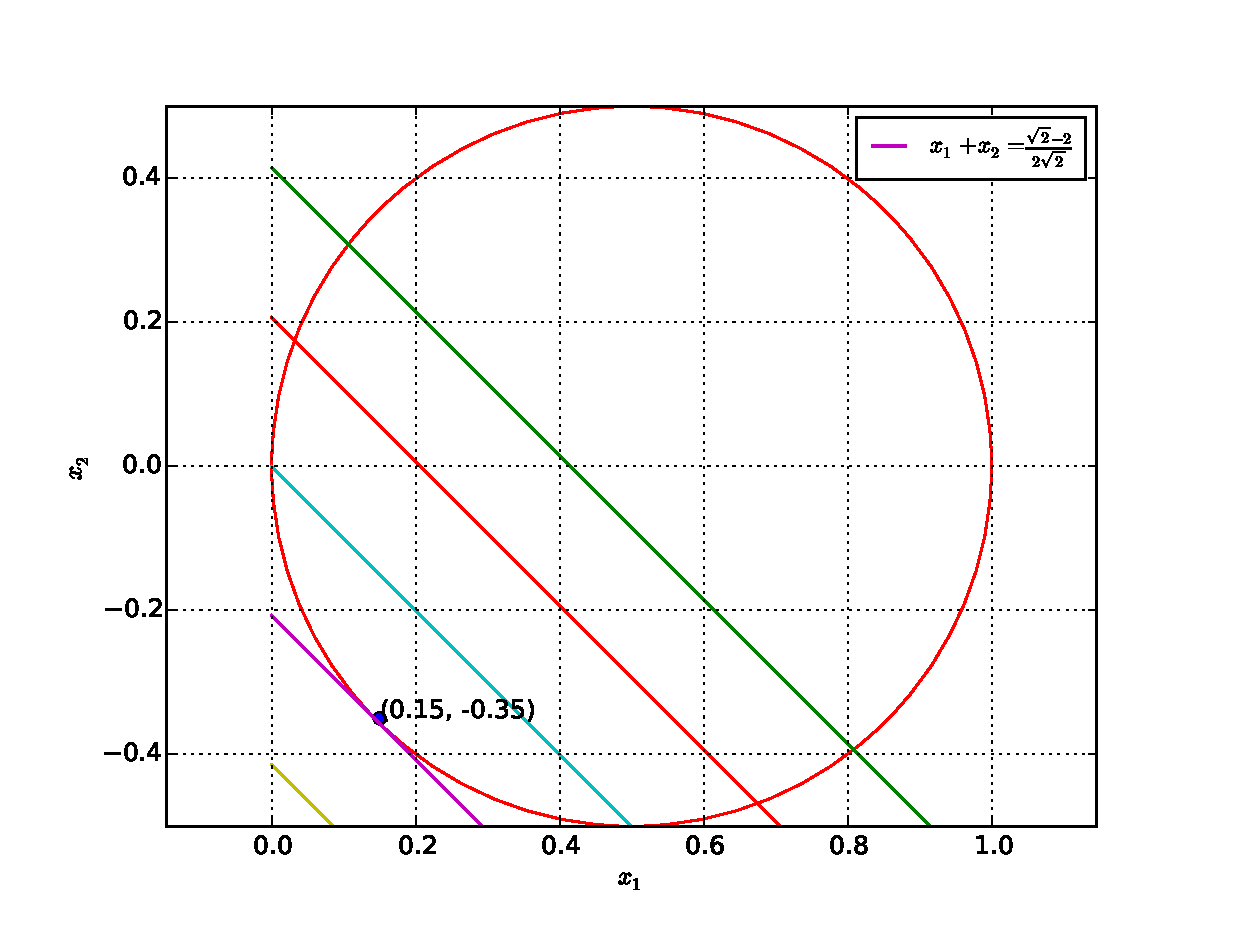
\includegraphics[width=\columnwidth]{./figs/2.15.eps}
%\caption{ Optimal solution is the lower tangent to the circle}
%\label{fig.2.15}	
%\end{figure}
%

%\subsection{Karush Kuhn-Tucker Conditions}

\item
%
\label{prob:cvxopt}

%\label{ch3_convex_ch2}
The problem
\begin{equation}
\min_{\mbf{X}} x_{11} + x_{12}
\end{equation}
%	
with constraints
\begin{align}
x_{11} + x_{22} &= 1 \\	
\mbf{X}
& \succeq 0 \quad  \brak{\text{$\succeq$ means positive definite}}
\end{align}
%
where
\begin{equation}
\mbf{X}=
\begin{pmatrix}
x_{11} & x_{12} \\
x_{12} & x_{22}
\end{pmatrix} 
\end{equation}
%
is known as a semi-definite program. 

%\solution The {\em cvxopt} solver needs to be used in order to find a numerical solution.  For this, the given problem has to be reformulated as
%\begin{align}
%&\min_{\mbf{x}}  
%\begin{pmatrix}
%1 & 1 & 0
%\end{pmatrix}
%\begin{pmatrix}
%x_{11} 
%\\
%x_{12}
%\\
%x_{22}
%\end{pmatrix}
%\quad \text{s.t}
%\\
%&
%\begin{pmatrix}
%1 & 0 & 1
%\end{pmatrix}
%\begin{pmatrix}
%x_{11} 
%\\
%x_{12}
%\\
%x_{22}
%\end{pmatrix}
%=1
%\end{align}
%\begin{multline}
%x_{11}
%\begin{pmatrix}
%-1 & 0 
%\\
%0 & 0
%\end{pmatrix}
%+
%x_{12}
%\begin{pmatrix}
%0 & -1
%\\
%-1 & 0
%\end{pmatrix}
%+x_{22}
%\begin{pmatrix}
%0 & 0 
%\\
%0 & -1
%\end{pmatrix}
%\\
%\preceq 
%\begin{pmatrix}
%0 & 0 
%\\
%0 & 0
%\end{pmatrix}.
%\end{multline}
%%
%The following script provides the solution to this problem.
%\begin{lstlisting}
%wget https://raw.githubusercontent.com/gadepall/optimization/master/manual/codes/3.1.py
%\end{lstlisting}
%
\item
Frame Problem \ref{prob:cvxopt} in terms of matrices.

\solution
It is easy to verify that
\begin{equation}
x_{11} + x_{12} = 
\begin{pmatrix}
1 & 1
\end{pmatrix}
\mbf{X}^{T}
\begin{pmatrix}
1 
\\
0
\end{pmatrix}
\end{equation}
and
\begin{equation}
x_{11} + x_{22} = 
\begin{pmatrix}
1 & 0 & 0 & 1
\end{pmatrix}
\begin{pmatrix}
\mbf{X} & \mbf{0} \\
\mbf{0} & \mbf{X}
\end{pmatrix}
\begin{pmatrix}
1
\\
0 
\\
0
\\
1
\end{pmatrix}
\end{equation}
%
Thus, Problem \ref{prob:cvxopt} can be expressed as
\begin{equation}
\begin{split}
\min_{\mbf{X}} 
\begin{pmatrix}
1 & 1
\end{pmatrix}
\mbf{X}^{T}
\begin{pmatrix}
1 
\\
0
\end{pmatrix}
& \quad s.t
\\
\begin{pmatrix}
1 & 0 & 0 & 1
\end{pmatrix}
\begin{pmatrix}
\mbf{X} & \mbf{0} \\
\mbf{0} & \mbf{X}
\end{pmatrix}
\begin{pmatrix}
1
\\
0 
\\
0
\\
1
\end{pmatrix}
&=1,
\\
\mbf{X}
 & \succeq 0 
\end{split}
\label{prob:cvxpy}
\end{equation}
%	
\item
Solve \eqref{prob:cvxpy} using {\em cvxpy}.
 Compare with the solution 
in problem  \ref{convex_sdp_eqiv}.

%
\solution
\begin{lstlisting}
wget https://raw.githubusercontent.com/gadepall/optimization/master/manual/codes/3.1-cvx.py
\end{lstlisting}

\item
Minimize 
\begin{equation}
-x_{11} - 2x_{12} - 5x_{22}
\end{equation}
subject to
\begin{align}
\label{ch3_lin_mat_ineq_const}
2x_{11} + 3x_{12} + x_{22} &= 7 \\
x_{11} + x_{12} &\geq 1 \\
x_{11}, x_{12}, x_{22} &\geq 0 \\
\begin{pmatrix}
x_{11} & x_{12} \\
x_{12} & x_{22}
\end{pmatrix} & \succeq 0 
\end{align}
using {\em cvxpy}.

%\solution
%In this problem, there is an SDP inequality and several linear inequalities.  The linear inequalities can be combined to obtain the matrix inequality
%%
%\begin{equation}
%\label{ch3_lin_mat_ineq}
%\begin{pmatrix}
%x_{11} + x_{12}- 1 & 0  & 0 & 0\\
%0 & x_{11} & 0 & 0
%\\
%0 & 0 & x_{12} &  0
%\\
 %0 & 0 & 0 & x_{22} 
%\end{pmatrix}
 %\succeq 0 
%\end{equation}
%%
%\eqref{ch3_lin_mat_ineq} can be combined with the matrix inequality in \eqref{ch3_lin_mat_ineq_const} to obtain the composite SDP
%\begin{equation}
%\label{ch3_lin_mat_sdp_ineq}
%\begin{pmatrix}
%\begin{matrix}
%x_{11} + x_{12}- 1 & 0  & 0 & 0\\
%0 & x_{11} & 0 & 0
%\\
%0 & 0 & x_{12} &  0
%\\
 %0 & 0 & 0 & x_{22} 
%\end{matrix}
%& \mbf{0}
%\\
%\mbf{0} & \begin{matrix}
%x_{11} & x_{12} \\
%x_{12} & x_{22}
%\end{matrix}
%\end{pmatrix} 
 %\succeq 0 
%\end{equation}
%%
%For using  {\em cvxpy}, the SDP in \eqref{ch3_lin_mat_sdp_ineq} can be expressed as
%%
%\begin{equation}
 %x_{11}F_{0} + x_{12}F_1+x_{22}F_{2}\succeq B ,
%\end{equation}
%%
%where
%%
%\begin{align}
%F_{0} = 
%\begin{pmatrix}
%\begin{matrix}
%1 &
%\\
%& 1
%\end{matrix}
%& & \bigzero
%\\
%& 
%\begin{matrix}
%0 &
%\\
%& 0
%\end{matrix}
%&
%\\
%\bigzero& & 
 %\begin{matrix}
%1 &  \\
 %& 0
%\end{matrix}
%\end{pmatrix} 
%\\
%F_{1} = 
%\begin{pmatrix}
%\begin{matrix}
%1 &
%\\
%& 0
%\end{matrix}
%& & \bigzero
%\\
%& 
%\begin{matrix}
%1 &
%\\
%& 0
%\end{matrix}
%&
%\\
%\bigzero& & 
 %\begin{matrix}
%0 & 1 \\
%1 & 0
%\end{matrix}
%\end{pmatrix} 
%\\
%F_2 = 
%\begin{pmatrix}
%\begin{matrix}
%0 &
%\\
%& 0
%\end{matrix}
%& & \bigzero
%\\
%& 
%\begin{matrix}
%0 &
%\\
%& 1
%\end{matrix}
%&
%\\
%\bigzero& & 
 %\begin{matrix}
%0 &  \\
 %& 1
%\end{matrix}
%\end{pmatrix} 
%\end{align}
%and
%\begin{align}
%B=
%\begin{pmatrix}
%\begin{matrix}
%1 &
%\\
%& 0
%\end{matrix}
%& & \bigzero
%\\
%& 
%\begin{matrix}
%0 &
%\\
%& 0
%\end{matrix}
%&
%\\
%\bigzero& & 
 %\begin{matrix}
%0 &  \\
 %&0
%\end{matrix}
%\end{pmatrix} 
%\end{align}
%%
\item
	Repeat the above exercise by converting the problem into a convex optimization problem in two variables and using graphical plots.  

\item
	Solve the above problem using the KKT conditions.  Comment.

\end{enumerate}
